\chapter{Численные методы и комплексы программ}\label{ch:ch3}


\section{Первая статья}\label{sec:ch3/sect1}


Пусть функционал $J(\theta)$ удовлетворяет условиям, указанным в \autoref{sec:optimality}.
Для удобства введём переобозначение $\hat{J}(u):=J(\theta(u)), \hat{J}:L^2(\Gamma_1) \to \mathbb{R}$.
Здесь $\theta(u)$ -- температурное поле задачи  \eqref{initial}--\eqref{initial-boundary} отвечающее
управлению $u \in L^2(\Gamma_1)$.
Согласно формуле \eqref{therorem_2_eq3} градиент функционала $\hat{J}(u)$~\cite{grenkin_13} имеет вид
\[
    \hat{J}'(u)= (\varphi(u) -\theta_b^4)p_2,
\]
где $\varphi(u)$ есть интенсивность излучения, $p_2$ -- соответствующая переменная сопряжённой системы.

Предлагаемый алгоритм решения выглядит следующим образом:
\begin{algorithm}[H]
    \caption{Алгоритм градиентного спуска с проекцией}
    \begin{algorithmic}[1]
        \State Выбираем значение градиентного шага $\lambda$,
        \State Выбираем количество итераций $N$,
        \State Выбираем произвольное $u_0 \in U_{ad}$,
        \For{$k \gets 0,1,2,...,N$}
            :
            \State Для полученного $u_k$ расчитываем состояние $y_k = \{\theta_k, \varphi_k\}$ из  (\ref{weak_operational}).
            \State Расчитываем значение функционала качества $J(\theta_k)$ из (\ref{quality}).
            \State Расчитываем сопряжённое состояние $p_k=\{p_{1k},p_{2k}\}$ из уравнений \eqref{therorem_2_eq1}--\eqref{therorem_2_eq2}, где $ \hat{\theta} := \theta_k, \hat{u}=u_k$.
            \State Пересчитываем управление $u_{k+1} = P_{ad}\left[ u_k - \lambda (\varphi_k - \theta_b^4)p_{2k} \right]$.
        \EndFor
    \end{algorithmic}\label{alg:algorithm}
\end{algorithm}
Оператор проекции $P_{ad} : U \to U_{ad}$ определён следующим образом
\[
    P_{ad}[v] =
    \begin{cases}
        u_1, & \text{если } v \le u_1 \\
        v, & \text{если } u_1 < v < u_2 \\
        u_2, & \text{если } v \ge u_2
    \end{cases}
\]
Приведём далее примеры расчётов для двумерного случая.
Положим $\Omega = \{(x,y), 0 \leq x,y \leq 1\}$, $l = 1$ см.
Граница $\partial\Omega$ состоит из участков:
\[
    \begin{aligned}
        \Gamma_0 & = \{x=\{0,1\}, y \in [0,1]\} \\
        \Gamma_1 & = \{x\in [0,1], y=0\} - \text{участок с неизвестными отражающими свойствами,} \\
        \Gamma_2 & = \{x \in [0,1], y=1\} - \text{участок наблюдения.}
    \end{aligned}
\]
Будем также далее считать, что $a = 0.006[\text{см}^2/\text{c}]$, $b=0.025[\text{см}/\text{с}]$, $\beta = 0.00005[\text{см}/\text{с}]$, $\kappa=1[\text{см}^{-1}]$, $\kappa_s = 0$, $A = 0$, $\gamma = 0.3$.
Указанные параметры соответствуют стеклу \cite{grenkin_13}.
Температуру на границе $\Omega$ положим равной $\theta_b = (x^2+y^2)/3$.

При указанных параметрах для первого эксперимента выберем следующее тестовое значение
функции $u$ (рис. \ref{fig:control}\subref{fig1:exp1}):
\begin{equation}
    u(x)=
    \begin{cases}
        0.01, & \text{если } x \le 0.5, \\
        0.5, & \text{если } x > 0.5,
    \end{cases}\label{eq:equation}
\end{equation}
и для второго эксперимента (рис.~\ref{fig:control}\subref{fig1:exp2}):
\begin{equation}
    \label{eq:test_function_1}
    u(x)=0.49x+0.01. \;
\end{equation}

Вычислим решение прямой задачи~\eqref{eq:initial}--\eqref{eq:initial-boundary} для этих случаев.
Полученное температурное поле на участке наблюдения $\Gamma_2$ выберем в качестве $\theta_0$.
Далее, применяя предложенный алгоритм находим квазирешение
обратной задачи~\eqref{eq:initial}--\eqref{eq:theta_gamma}.
Эффективность алгоритма, а также значение $u_0$ в первом и
втором случаях иллюстрируются рис.~\ref{fig:control}.
На рис.~\ref{fig:cost} показана динамика функционала качества по итерациям.

\textbf{Замечание.} В предложенных примерах потребовалось $2*10^6$ итераций для нахождения квазирешения $u$.
В то же время температурное поле на участке наблюдения $\Gamma_2$ становится близким
к $\theta_0$ уже на $10^2$ итерации.
Также наблюдается существенное падение скорости уменьшения функционала качества с
каждой итерацией после того, как среднее значение найденной функции контроля
становится близко к тестовой функции.
\begin{figure}[H]
    \centering
    \subfloat[Первый эксперимент]
    {
        \label{fig:exp1}
        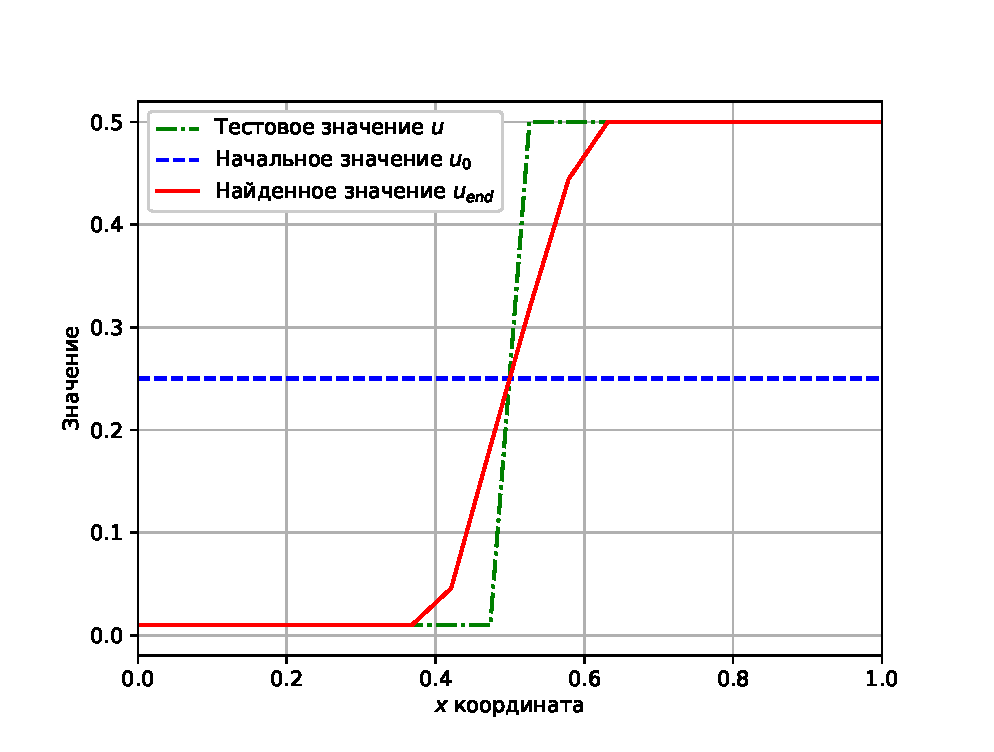
\includegraphics[width=.51\linewidth]{1.eps}
    }
    \subfloat[Второй эксперимент]
    {
        \label{fig:exp2}
        \includegraphics[width=.51\linewidth]{2.eps}
    }
    \caption{Тестовая функция $u$, начальная $u_0$, найденная функция $u_{end}.$}
    \label{fig:control}
\end{figure}

\begin{figure}[H]
    \centering
    \subfloat[Первый эксперимент]
    {
        \label{fig:exp12}
        \includegraphics[width=.51\linewidth]{3.eps}
    }
    \subfloat[Второй эксперимент]
    {
        \label{fig:exp22}
        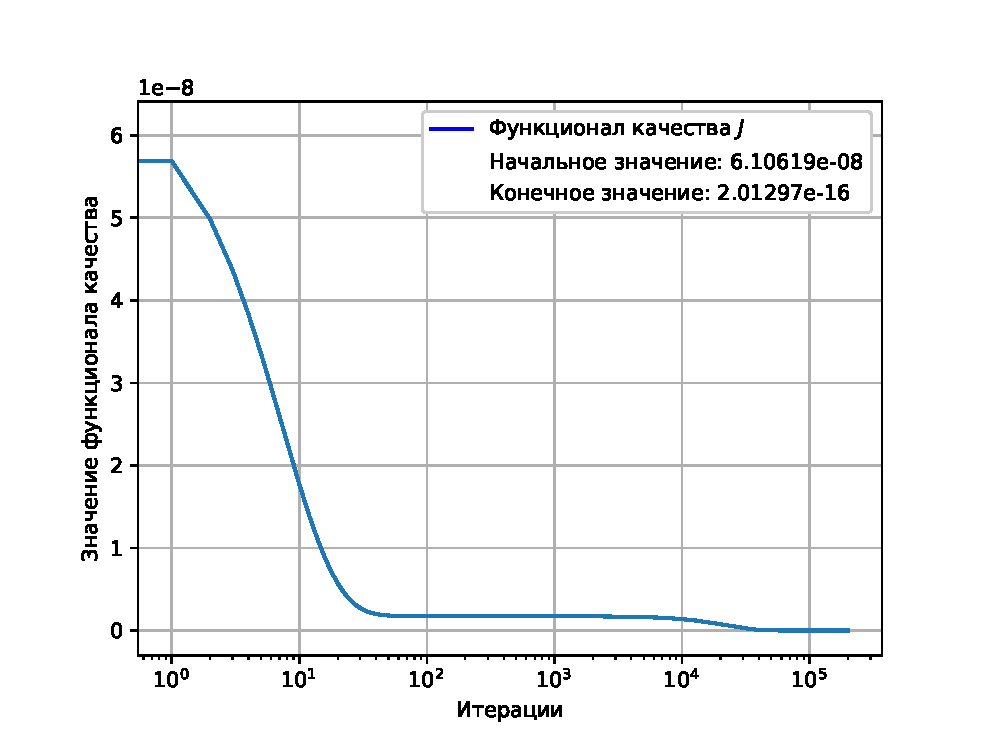
\includegraphics[width=.51\linewidth]{4.eps}
    }
    \caption{Динамика функции $\hat{J}(u)$ по итерациям.}
    \label{fig:cost}
\end{figure}

\clearpage
